\section{Results}
\subsection{Model Performance}\label{subsec:model-performance}
Overall, the models developed as part of the intelligence hierarchy performed fairly well.
\autoref{fig:apple-tree-mode-training-curve} demonstrates a learning curve for one of the first-layer apple-in-view models.
The model was able to learn in fairly few epochs, and seemed to achieve fairly low loss.
A confusion matrix was then generate on a test set, the results of which can be seen in \autoref{fig:apple-in-view-confusion-matrix}.

\begin{figure}[!htb]
    \centering
    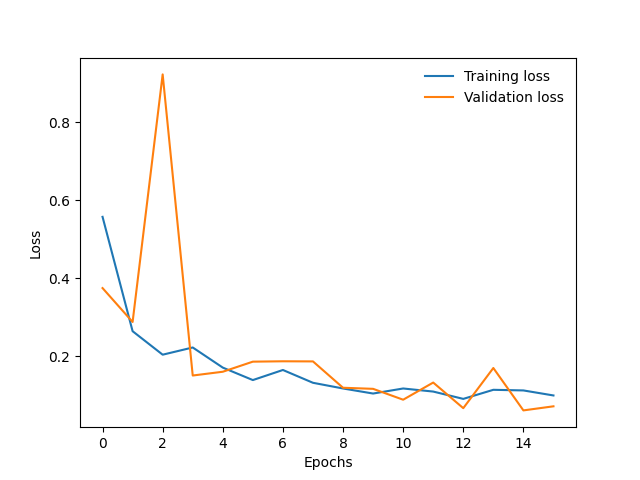
\includegraphics[width=\columnwidth,keepaspectratio]
    {./figures/mobile_model_apple_trees_16its_2022-11-15_training_curve}
    \caption{
        Learning curve for a apple-in-view CNN.
        The model is a retrained version of MobileNet~\cite{Sandler2018,PyTorchMobileNet}, which is a more light-weight while still very powerful CNN.
        Loss is in mean squared error.
    }
    \label{fig:apple-tree-mode-training-curve}
\end{figure}

\begin{figure}[!htb]
    \centering
    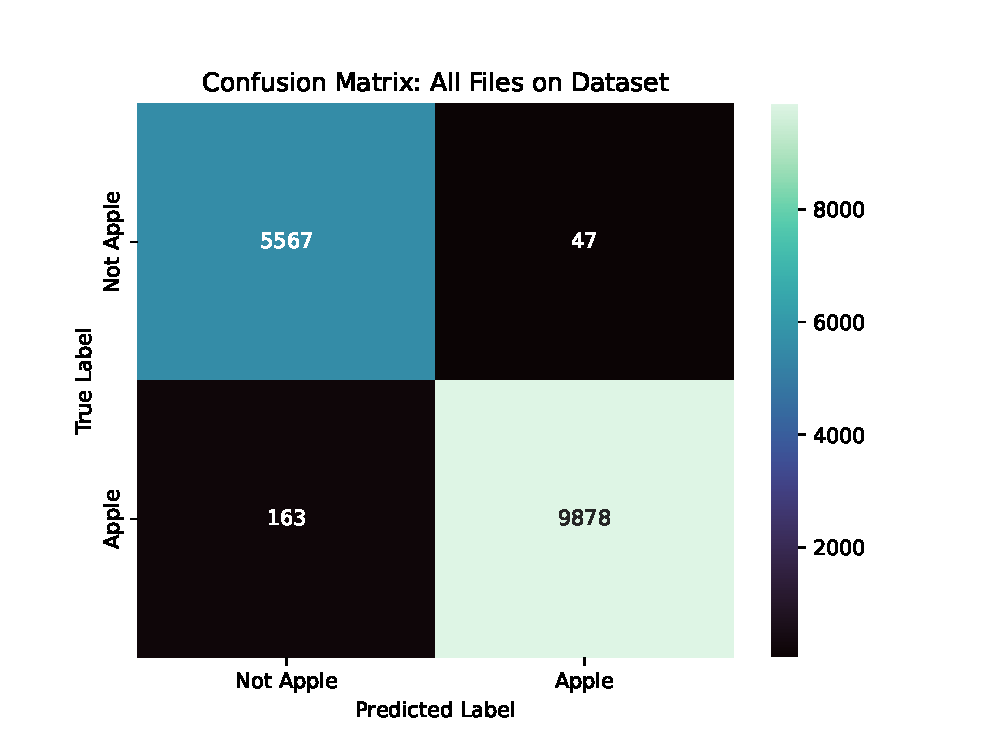
\includegraphics[width=\columnwidth,keepaspectratio]
    {./figures/confusion_matrix_All_Files_on_Dataset}
    \caption{
        The confusion matrix of the primary apple-in-view detection model on a test set.
        The column is the predicted label, while the row is the true label.
        A perfect model will have 0s in the top-right and bottom-left corner.
    }
    \label{fig:apple-in-view-confusion-matrix}
\end{figure}

While these initial models appear to perform well, as second round of tests from a small, separate dataset consisting of hands holding apples was conducted and yielded considerably worse results (see \autoref{fig:apple-in-hand-confusion-matrix}).
This is not only true for the apple-in-view layer models, but models at all levels of the intelligence hierarchy.
We believe this is because the datasets used to train the models~\cite{Fruit360,Sultana2022} may not have been sufficiently diverse.
We attempted to enhance the dataset through curating web-scraped images, but the models ultimately yielded the same results. Although we experienced a decent amount of success using this model, we lacked the data, training time, and compute capacity to create a model that was consistently performant.
Given more time, we feel better data could be accumulated and better models developed.

\begin{figure}[!htb]
    \centering
    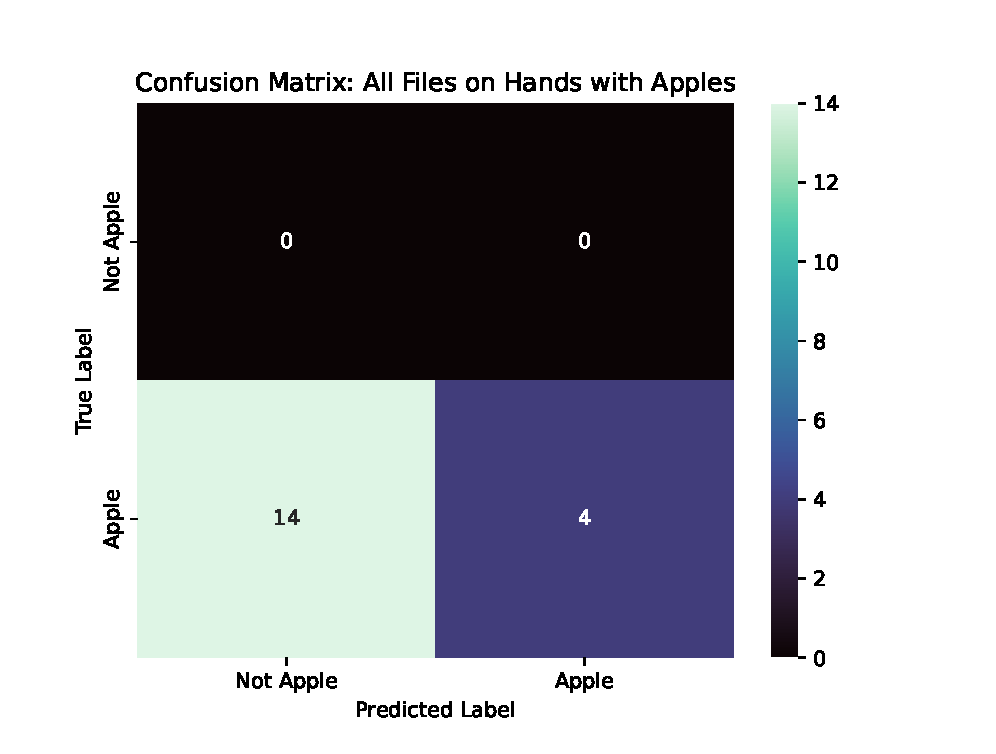
\includegraphics[width=\columnwidth,keepaspectratio]
    {./figures/confusion_matrix_All_Files_on_Hands_with_Apples}
    \caption{
        The confusion matrix of the primary apple-in-view detection model on a new, apples-in-hand dataset.
        The column is the predicted label, while the row is the true label.
        A perfect model will have 0s in the top-right and bottom-left corner.
        Notice how the model fails to correctly classify the majority of images.
    }
    \label{fig:apple-in-hand-confusion-matrix}
\end{figure}

\subsection{Robot Performance}\label{subsec:robot-performance}
Even with their shortcomings, the models developed were sufficient for use with the drone.
\autoref{fig:drone-haar-cascade} shows an image captured from the drone during its movement phase.

\begin{figure}[!htb]
    \centering
    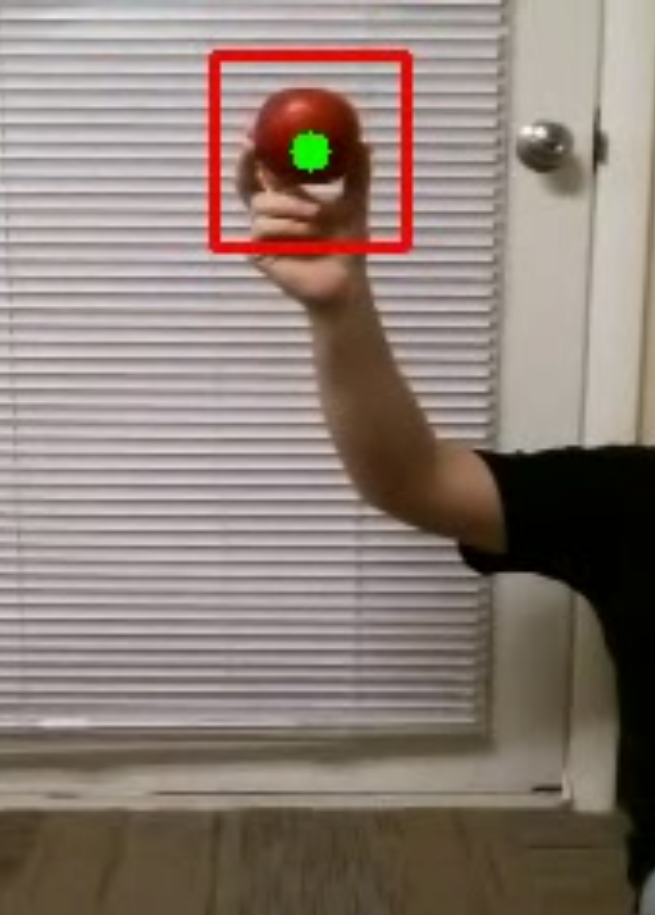
\includegraphics[width=\columnwidth,keepaspectratio]
    {./figures/haar-cascade-detection}
    \caption{
        An image taken through the drone camera during the calculate-relative-position phase of the intelligence hierarchy.
        A Haar-Cascade model is used to identify the apple's location and distance relative to the drone, after which the drone is able to approach the apple.
    }
    \label{fig:drone-haar-cascade}
\end{figure}
